\chapter{О горах и ведьмах}

В этой части книги я хотел собрать сведения обо всех киевских Лысых горах, да так вышло, что про большинство из них уже рассказал.

Вообще Лысых гор по свету разбросано много – так называют всякую плешивую сверху возвышенность. Неско\-лько меньше холмов, о которых ходила дурная молва как о местах сходбища нечистой силы, проведения шабашей. Например, в Германии есть гора Броккен\footnote{В 20 веке, долгое время на ней располагались военные объекты разных стран, а сейчас – телевышка, гостиница и музей.}, куда под Вальпургиеву ночь слетались ведьмы на шабаш.  Недобрые слухи ходили и про многочисленные Бабьи горы.

%Существует Лысая гора в Рязани, в Самаре (часть Сокольих гор), множество даже городов и сел носят такое название.

Основным местом шабашей на Руси славилась Лысая гора «под Киевом». Это звание может быть справедливо разделено между несколькими горами киевскими.

Но поначалу о роли, отводимой Лысой горе в преданиях. Народ верил, что туда в определенные ночи (например, под Ивана Купала) слетаются ведьмы и упыри, молодые и старые. Невежды в демонологии ставят знак равенства между вампиром образца Дракулы и славянским упырем. Между тем, согласно поверьям, упырь – или, иначе, ведьмач – это колдун, старший над ведьмами в определенной местности. Мертвый упырь будто может бродить по ночам и пить кровь, предпочитая употреблять её из пальца и у младенцев. Живой упырь же отличается крепким здоровьем и румяностью – внешне противоположен тем бледным чахликам, коих нам подсовывает киноиндустрия.

В народе ходили былички о нечистой силе. Некоторую их долю составляли рассказы о ведьмах. Случайный человек, например солдат, останавливается переночевать у женщины, она оказывается ведьмой. Герой наблюдает, как она варит некий отвар, мажет им у себя под мышками и улетает в печную трубу. Герой повторяет те же действия и устремляется следом, на Лысую гору. Другой распространенный сюжет – герой женится, а жена его, купно со тещей, оказываются ведьмами.

Среди литературных обработок таких быличек – «Киевские ведьмы» Ореста Сомова, «Вий» Гоголя. В «Вие» кстати много чего выдуманного или неприсущего нашему краю, например гномы и сам Вий. Были, впрочем, подобные Вию существа. Про Шолудивого Боняка я уже говорил, а еще припомним святого Касьяна, который, согласно поверьям, появлялся 29 февраля и обладал смертельным взглядом, отчего крестьяне старались не покидать жилищ в тот день високосного года.

%Ходили былички и совершенно дикие, впору тогдашним нравам. Крестьянин встречает некое животное, калечит его, а наутро в селе находят искалеченную, исходящую кровью старуху и смекают – ага, ведьма! Ничем, кроме пьяной дикости или злой клеветы, такие истории объяснить нельзя.

Ведьм различали на врожденных и ученых. Врожденные были как бы изначальными носителями неких знаний и способностей, а также имели небольшой хвост и полоску шерсти вдоль позвоночника. А ученые, или наученные ведьмы – это обычные женщины, которых обучили колдовству. Последние считались более склонными ко злу, нежели врожденные. Врожденные же могли исправлять плоды козней ученых ведьм.

Вера в ведьм и упырей не была исключительно сельской – городские суды (вплоть до начала 19 века) разбирали взаимные обвинения в ведовстве, в различных колдовских действиях, направленных на причинение вреда. В сельской местности поступали иначе – избивали, жгли, топили заподозренных. Обвинить человека в колдовстве могли просто корысти ради, скажем, из-за спорной земли.

Способы выявления ведьм и упырей соревновались друг с другом в жестокости, причем смертоносную дурь какого-нибудь одного «знатока», охочего до причинения другим увечий, поддерживала толпа. Иван Франко в работе «Сожжение упырей в Нагуевичах» сообщает, как живых людей таскали через костёр, чтобы отыскать среди них упыря. А вот что пишет Чубинский в томе первом «Трудов этнографическо-статистической экспедиции в Западно-русский край»\cite{trudy-chub}:

\begin{quotation}
[Луцкий уезд]. Рассказывают, что в одном месте не было долго дождя, а потом помещик велел собрать всех женщин и класть их спиной в воду, придерживая веревкой; которая из них будет тонуть – ту вытаскивать, а которая будет плавать на поверхности – ту бить, потому что она ведьма. Одна из женщин оказалась такою; когда ее начали бить, то полился такой дождь, что люди, едва живы, дошли домой.
\end{quotation}

Жаль, что не начали бить самого помещика. Тогдашние представления о причинно-следственном механизме мироздания отражает народная медицина. Как раньше лечили лихорадку? Из тех же «Трудов»:

\begin{quotation}
Смешивают испражнение свиньи с медом и дают больному.

Спящему кладут лягушку за пазуху.

Больной закапывает яйцо в могилу и ложится туда же спать. Проснувшись утром, выпивает закопанное яйцо.

Больной, три ночи сряду, отправляется ночевать в свинарню. Ночью к нему будет являться женщина и будет просить уступить ей место; если он не исполнит ея просьбы, – будет здоров!

Взять у больного три вши и секретно дать ему их выпить с водой.
\end{quotation}

Ведьмы и упыри всегда оказывались в представлении народа «крайними», виноватыми во всех бедах – будь то засуха, болезни людей и животных, хотя к ним же прибегали, за неимением врачей, за помощью, как и к колдунам-знахарям и знахаркам, иначе говоря «бабкам». От последних народ отличал ведьм тем, что бабки не имели способности к оборотничеству, полетам и тому подобному, хотя порой представления о бабках и ведьмах смешивались.

Меня в детстве водили к бабке, чтобы избавить от заикания. Это было весной 1986 года, когда мы с моей бабушкой Таней спешно, спасаясь от чернобыльской радиации, уехали из Киева к практически незнакомым людям в село Кротенки\footnote{В 2016 году ей вернули исконное название, Семьяновка.}, под Полтаву. Там чудесная природа. Громадный холм, под ним раскинулось село на берегу тихой речки Ворсклы, а на другом ее берегу, через просторное поле, в пяти километрах синел лес, где среди деревьев горел факел газовой скважины.

На горе росли кусты терновника, да могучий древний дуб, достойный кисти Шишкина. По травянистому склону выпасали коров. Вниз шла крутая грунтовка, и если спускаться нею, то слева тянулось кладбище\footnote{49°40'25.4"N 34°35'12.7"E}. Рассказывали, что однажды корова, взбесившись, бегала там и сворачивала рогами кресты.

На половине горы, ближе к низу, под кладбищем, находился уступ. И там в кривенькой хатке жила «бабка». Рядом с калиткой в ее двор был знаменитый на всю округу 15-метровый колодец с очень вкусной и студёной, до боли в зубах, водой. Надо было долго крутить ворот со звенящей цепью, чтобы поднять из темени ведро.

Бабка приняла нас безо всякой предварительной договоренности, как само собой разумеется. Пришли незнакомые люди, а она поняла, зачем. Маленькая, сухонькая, сгорбленная, лицо под косынкой всё в глубоких морщинах, и конечно же крючковатый нос – всё как полагается.

Она оставила мою бабушку в прихожей, а меня отвела в комнатку, где посадила на табурет, а сама что-то намешала в посудинке и, попросив меня закрыть глаза, стала «шептать». Я расслышал отдельные слова: «будут и машины, будут и тракторы». Я подсматривал краем глаза, но головой не крутил, чтобы не стало заметно. Бабка лила в посуду расплавленный воск и он застывал в каких-то образах, очевидно значащих для ведуньи.

Потом она вернула меня в прихожую. От людей мы с бабушкой знали, что «бабка» берет оплату конфетами, и дав ей свои конфеты, поняли, зачем. Взамен «бабка» тоже наделила нас конфетами – несколько шоколадных – «Белочка», еще длинные такие с лещиной, да сосательные леденцы барбариски.

Хотя от заикания она меня не исцелила, в памяти остался положительный образ бескорыстного человека. Может, она кому-то помогала, особенно, наверное, если человек верил в ее силу.
 
Большинство известных популярно сведений о шабашах, что кочуют по статьям и книгам, были вырваны клещами европейской инквизиции у ее жертв. Поэтому я не рассматриваю такие сведения, считая их выдумкой.

У нас же в народе верили, что на шабаш под Киев ведьмы слетались по крайней мере трижды в год – на Коляду, Юрьев день\footnote{Мой день рождения, 6 мая.} да в ночь накануне Ивана Купала. Иван Купала – это Иоанн Креститель\footnote{Обряд отпущения грехов он, как ныне христиане – крещение, проводил купанием.}. «Ивановой ночи» вообще придавалось огромное колдовское значение – в нее люди собирали чародейские травы: тирлич, архил\'ин, искали цветок папоротника, проявляла себя «нечистая сила».

День рождества Иоанна Крестителя отмечался 24 июня по «старому стилю», по юлианскому календарю. Согласно используемому нами григорианскому календарю это, в 20-21 веках, 7 июля (24+13 дней), а в 22 веке уже 8 июля, надо прибавлять 14 дней. Иными словами, счет дней по юлианскому календарю отстает от счета дней по григорианскому календарю, и величина этого запаздывания из века в век растет.

У разных календарей, и юлианского и григорианского, есть погрешности относительно астрономических явлений, по которым можно судить о ходе дней, смене времен года – равноденствия, летнего и зимнего солценостояний. Григорианский календарь был разработан в 1582 году потому, что к тому времени, за века, прошедшие со введения Юлием Цезарем юлианского календаря, накопившаяся в последнем погрешность составила 10 суток относительно весеннего равноденствия. Григорианский календарь отбросил эти 10 суток и ввел свои правила счета лет.

На 21-22 июня по григорианскому календарю приходится астрономическое явление – солнцестояние, солнцеворот. Это самая короткая ночь в году, после чего светлое время суток начинает уменьшаться до зимнего солнцестояния, 21-22 декабря – когда самый короткий световой день.

Очевидно, что многие народные праздники, приуроченные к христианским, отмечаются кроме прочего с обрядами исконными – поганскими, языческими. Все эти куличи, писанки, прыжки через костры, завивание венков, разбрасывание травы – это же не христианское учение предписывает делать.

И считается, что языческие праздники были привязаны к астрономическим явлениям. Полагают, что в поганском обществе существовал какой-то связанный с летним солнцестоянием праздник. После принятия христианства, на сей языческий праздник наложился церковный – день рождения Иоанна Крестителя, или, как его назвали в народе, Ивана Купалы\footnote{Обычай «купальских огней» присущ также населению Ирландии, где этот праздник называют Saint John Eve, канун святого Джона, Иоанна. Ирландцы зажигали на холмах костры, плясали вокруг, а затем прыгали через огонь.}.

Неведомо, каким календарем пользовались давние Славяне-погане\footnote{Возможно он был лунным, либо использовалось сразу несколько календарей. Даже в христианские времена, в летописях находим любопытное – например, такая запись (по Лаврентьевскому списку): «В лето 6615, индикта, круг луны 4 лето, а солнечнаго круга 8 лето. В се же лето преставися Воломидеряя, месяца мая в 7 день.». Или «В лето 6621. Бысть знаменье в солнци в 1 час дне, бысть видити всем людем, остася солнца мало аки месяца долов рогома, месяца марта в 19 день, а луны в 9».}. Праздник Ивана Купала, некогда получив привязку к календарю юлианскому, начал сдвигаться относительно астрономического солнцестояния – своего предполагаемого поганского дня празднования.

В 19 веке, когда фольклористами и были собраны основные сведения об этом празднике, день, в который его отмечал народ – 24 июня по принятому тогда юлианскому календарю – почти на две недели отставал от настоящего солнцестояния!

Эту привязку к юлианскому календарю следует учитывать при рассуждении обо всех народных праздниках, не говоря уже о тех, дата коих привязана к Пасхе и поэтому «плавает» от года к году.

Но ведь праздники обросли множеством поверий. Допустим, в Иванову ночь ведьмы слетаются на Лысую гору. Тогда же цветет папоротник. И если ведьмы – часть населения – как и все придерживались юлианского календаря, сложно заподозрить в этом цветок папоротника или каких-нибудь чертей.

Есть только два варианта оценки записанных в 19 веке верований (для удобства рассуждений примем их за истинные), связанных с любым народным праздником.

Первый – поскольку день праздника более не соответствует времени предполагаемого поганского «астрономического» праздника, то сопутствующие предания ошибочно, несправедливо приписаны дню юлианского календаря. С поправкой – все или часть поверий. Повторюсь, ведьмы как часть человеческого общества наверняка придерживались юлианского календаря. Наступает календарный Ивана Купала – накануне летят ведьмы на Лысую гору.

Второй – придется отрицать связь простейших для наблюдения астрономических явлений с давними поганскими праздниками, и искать какие-то другие астрономические закономерности, которыми пользовались погане для счета времени. Быть может это те же закономерности, что положены в основу юлианского календаря.

А можно не заморачиваться и рассуждать без чудесной составляющей поверий, тогда вся эта связанная с Ивановой ночью чертовщина – выдумка. Однако два приведенных выше варианта, хоть без летающих ведьм, однако с прыжками через костры, остаются в силе.

На Руси, 23 июня по старому стилю, в некоторых местах был слыло «Купальницами», «Купалом» или как «Аграфены-купальницы» – день всеобщих купаний в водоемах и банях. У западных Славян, Ивановская ночь (с 23-го на 24-е) и связанные с нею обряды известна как Соботки.

Вероятно, в празднике Ивана Купала совместились два смежных давних праздника – Купала (вне связи с Иоанном Крестителем) и Соботки. На двухдневность указывают «купальские» песни, где в первой строке часто звучит: «Сегодня Купала, а завтра Ивана!»\footnote{Эту песню знают и на Подолье: «Цепер Купайло, заутра Йван, чорт хапае ведзьмы церэз баркан».}. Значит, Купало – день, предшествующий Ивану, а Иван это Креститель, хоть и тоже Купало. Поэтому оба дня, и 23, и 24 число по старому стилю, упрощенно назывались Иваном Купалой, с разницей, и обряды были распределены на два дня.

В первый, 23-го, основные «купальские» обряды это купания в воде, украшение венками срубленного дерева – его называли Купалом. В ночь на 24 – прыжки через огонь. 24-го же делали из соломы куклу по имени Морена, или Марина, Уляна, Катерина (разнится от местности). Ее считали «старшей русалкой». Морену наряжали в платье, украшали, носили по улицам, а потом к реке, где снимали с куклы украшения, а ее саму бросали в воду. Всё это с особыми песнями.

Так или иначе, в представлениях народа, эти два дня были связаны с ведьмами. Например на Полесье\cite{tolstaya01}, 23-е (6 июля по новому стилю) называли Ведьминым днем, ночь с 23 на 24-е – Ведёмская ночь, Ведьмарская ночь, Ведьмин вечер, Иванова ночь, Купайла, Купайло, Купальная ночь, Скакунов вечер, Страшная ночь, ап 24-е – Иван Ведёмский, Иван Ведьмак, Иван Ведьмарский, Иван Злостный, Иван Купала, Иван Колдунский, Иван Цветошин, Ян, Купайла, Иван Купальский, Янка Купала.

Название Соботок или Соботки используют Славяне западные, например Поляки, хотя и не все – на Подлясье и Мазовии ходило название «Купальночка». Даль в «Словаре» пишет, что по реке Луге на Новгородщине и Петербургщине, Ивана Купалы тоже слыло Соботкой, и предполагал, что это «от собить, готовить, припасать».

Но мне кажется более очевидной связь между словом «шабаш» и Соботкой.

Вообще-то, в народе не говорили о «шабашах», а рассказывали просто, мол, ведьмы летают на Лысую гору.

Однако познакомимся со словом «шабаш» ближе. 

С ним сходно слово «суббота», наш шестой день недели, и общепринято считать «субботу» искаженным «шаб\'ат» или «ш\'абос», как иудеи называют свой седьмой день недели, что в переводе означает «прекращение работы», «отдых» – поскольку согласно их да христианским верованиям, бог после шестидневного сотворения мира на седьмой день отдыхал.

Это решение вопроса с одной стороны. Но вот соображения с другой. 

Слова «Соботки» и «Соботка» проявляются среди славянских земель в названиях гор, городов и фамилиях. Известен древний город Сопот (С\'опот по-польски, и Соп\'от на местном кашубском наречии) в Польше, на берегу Балтийского моря.

Праздник Соботка, связанный с купанием, и старинный славянский обычай париться в бане по субботам. Была даже пословица «баня все грехи смоет» – а кстати Иван Креститель-Купала, как известно, смывал с людей грехи в воде. 

В 17 веке обычаю париться в банях именно по субботам церковь придавала значение поганского обряда и пыталась бороться с этим, что отражено в духовных и светских документах. В грамоте царя Алексея Михайловича шуйскому воеводе Змееву о Коляде, Усени и народных играх, 1649 года перечисляются «бесчинства», творимые народом в Москве и округе, в том числе такие:

\begin{quotation}
многие люди поют бесовския, сквернословныя песни, и против воскресных дней в субботу в вечеру, и в Господские и Богородичные дни топят бани
\end{quotation}

%Дни различных обрядовых поминок на Руси тоже справлялись обычно в субботу – Кормная суббота, Дмитриева (родительская) суббота, Званые поминки, Великая суббота\footnote{}. 

«Суботками» в народе называли и осенние посиделки со дня Покрова до половины ноября, а на Псковщине – святочные вечера, Святки. С этим временем в народе также связывались полеты на Лысую гору.

А сходство украинского слова «чобит» и русского «сапога»\footnote{А замените в «сапог» – «с» на «т» и «г» на «к», и получите «тапок».} с Соботкой меня вообще озадачивает. Кстати у Ильи Муромца было прозвище Чобиток.

%Собор. Собрание. Сборище. Что же такое «шабаш», как не сборище, собрание. Но у перечисленных выше слов корень «бор» – а «со» лишь приставка, обозначающая объединение. Со-ратник, со-единение. Вместе.

%Соботка. Событие.

%Со-батька?

На Ивана Купалу прыгают через костры. Удобнее делать это в сапогах, они прикрывают ногу до колена. В народе сапоги вообще носили, если летом, то больше для форсу – в грязь же разувались да ходили босиком.

П. В. Иванов в «Жизнь и поверья крестьян Купянского уезда, Харьковской губернии»\cite{ivanov01} писал о купальских игрищах:

\begin{quotation}
Перепрыгивают через огонь обыкновенно парами, парень с девкой, подростки же прыгают через крапиву без всякого порядка. Парень, сняв с девки венок, надевает ей на голову свою шапку, а себе ея венок, и, схватив девку за руку, прыгает с девкою через костер\footnote{В Минской губернии, в 19 веке, прыгали иначе – сначала одни только девушки, а кто не прыгал, ту называли ведьмой.}. Иногда же два парня, взяв девку с обеих сторон под руки, переводят через огонь, причем страдают не только юбка и сапоги, но нередко и ноги девки.
\end{quotation}

В первом томе «Народные южнорусские сказки» И. Рудченко, вышедшем в 1869 году, есть сказка «Чоботи», записанная в Васильковском уезде Киевской губернии. Начинается она с того, что умирающий богач, призвав к себе сына, завещает ему: «гляди ж, синку, щоб у тебе, як я и вмру, було так, як и в мене – що суботи були чобітки новенькі». И послушный сын заранее, каждую неделю в пятницу покупал себе новые сапоги и так разорился. Сказка впрочем о том, что отец-богач не сорил деньгами, а каждую субботу смазывал сапоги дегтем, и те выглядели новыми, однако – новые сапоги каждую именно субботу!

Что же могло означать слово Соботка, если искать в нем славянский корень? Прикинем. Сменим первую букву на «т», и получится Топотка. Топали, когда прыгали. А если Соботки таки связаны со словами «чобот» и «сапог»? В сапогах и прыгали, и плясали.

Возможно, купальские Соботки это охристианенный и немного приглушенный вариант ведьмовских лысогорских шабашей. На это намекают обряды. Например, есть поверье (без приурочивания к празднику), что ведьмы катаются по росе. А на Купалу в росе купались люди.

%И Коляда носила астрономическое значение, ибо, опять же более-менее, совпадала с зимним солнцестоянием. Позже Коляда, замещаемая христианскими праздниками, немного сдвинулась вперед по времени и стала обрядом накануне Рождества.

Кроме ночи накануне рождества Иоанна Крестителя, другие распространенные дни полетов на Лысую гору – под Великдень (Пасху) и под Воздвиженье.

По молве, чтобы отправиться на шабаш, ведьма действовала следующими способами. Варила какой-то отвар и натиралась под мышками, после чего вылетала в трубу. Либо – снимала с себя рубашку, намазывалась вся некой мазью, ставила в печь горшок с загадочной жидкостью, затем хватала помело или кочергу, садилась на него словно на лошадь и вместе с парами жидкости вылетала опять-таки через трубу. Или же кувыркались через воткнутый нож и – того, в небо по трубе.

О том, что именно происходило на шабашах, в народе знали смутно. Ведьмы и упыри плясали, пели, совершали какие-то странное игрушечное фехтование на палках, «тешились с чертями» – сведения различные и крайне отрывочные. Фольклорист Иван Петрович Сахаров в своем труде «Сказания русского народа» (изданном в 1830-х) поместил любопытные сведения по предмету, которые я привожу тут целиком:

\begin{quotation}
13. Песня ведьм на Лысой горе\\
\\
В заповедных сказаниях поселян есть поверие, что какой-то казак, забравшись на Лысую гору, подслушал песню ведьм; но шабашное сборище, узнавши об открытии, утопила казака в реке\footnote{Кому же казак передал песню перед смертью?}. С тех пор она гуляет по белу свету и передается чародеями одним только ведьмам\footnote{Пока Сахаров не поведал песню читателям.}. Нет почти никакой возможности постигнуть смысл этих слов. Это какая-то смесь разнородных звуков языка, никому не известного и, может быть, никогда не бывалого.
\end{quotation}

\settowidth{\versewidth}{А. а. а. – о. о. о. – и. и. и. – э. э. э. – у. у. у. – е. е. е.} 
\begin{verse}[\versewidth]
Кумара,\\
Них, них, запалам, бада,\\
Эшохомо, лаваса, шиббода.\\
Кумара.\\
А. а. а. – о. о. о. – и. и. и. – э. э. э. – у. у. у. – е. е. е.\\
Ла, ла, соб, ли, ли, соб, лу, лу, соб!\\
Жунжан,\\
Вихада, ксара, гуятун, гуятун,\\
Лиффа, пррадда, гуятун, гуятун, \\
Наппалим, вашиба, бухтара,\\
Мазитан, руахан, гуятун.\\
Жунжан.\\
Яндра, кулайнеми, яндра,\\
Яндра.
\end{verse}


\begin{quotation}
14. Шабашная песня ведьм\\
\\
Шабашная песня ведьм, говорят поселяне, открыта одною молодою девушкою, обращенною из ведьм в прежнее состояние.
\end{quotation}

\settowidth{\versewidth}{Веда, шуга, ла, на, да, шуга!} 
\begin{verse}[\versewidth]
Гутц!\\
Алегремос!\\
Астарот, бегемот!\\
Аксафат, сабатан!\\
Тенемос!\\
Гутц!\\
Маяла, на, да, кагала!\\
Сагана!\\
Веда, шуга, ла, на, да, шуга!\\
Сагана!\\
Гулла, гуала, на, да, лаффа!\\
Сагана!\\
Шиха, эран, рова!\\
Чух, чух!\\
Крыда, эхан, сцоха!\\
Чух, чух, чух!\\
Гутц!
\end{verse}

\begin{quotation}
15. Песня ведьм на роковом шабаше.\\
\\
Вот еще странное смешение звуков, сходное с выговором цыган. Пользуясь этою песнею, наши старухи-колдуньи думают, что обладают несметным богатством, что эта песня в состоянии сейчас обогатить того, кто только может пропеть ее. Замечательно, что эти старухи всегда бывают совершенно нищими, хотя находятся в состоянии петь по сту раз на день.
\end{quotation}

\settowidth{\versewidth}{Шию, шию, нетоли, – ба, ба, згин, ю.} 
\begin{verse}[\versewidth]

Шикалу, Ликалу!\\
Шагадам, магадам, викадам.\\
Небазгин, доюлазгин, фиказгин,\\
Бейхамаиш, гейлулашанн, эламаин.\\
Ликалу!\\
Шию, шию, дан, – ба, ба, бан, ю.\\
Шию, шию, нетоли, – ба, ба, згин, ю.\\
Шию, шию, бала, ли, ба, ба, дам, ю.\\
О вилла, вилла, дам, юхала!\\
Гираба, наюра, юхала!\\
Карабша, гултай, юхала!\\
Захива, ванилши, схабатай, янаха.\\
Захива, гиряй, гиряй, добила, янаха.\\
Захива, вилхомай, вилхомай, янаха.\\
Мяу! згин, згин!\\
Гааш! згин, згин!\\
У-у-у! згин, згин!\\
Бя – бая! – згин, згин!\\
Кво – кво! згин, згин!\\
Бду, бду! згин, згин!\\
Карра! згин, згин!\\
Тили, тили! згин, згин!\\
Хив, чив! згин, згин!\\
Жу, жу! згин, згин!\\
Згин, згин, згин!
\end{verse}

Подобна звучанием и: 

\begin{quotation}
16. Чародейская песня русалок.\\
 
Поселяне, приписывая русалкам обаятельную силу над молодыми людьми, скрывают за тайну чародейскую песню русалок, приводящую в усыпление. Звук слов этой песни совершенно непонятен, не говоря уже о значении. До сих пор еще люди, знающие всю подноготную, не умеют пользоваться этой песнию.
\end{quotation}

\settowidth{\versewidth}{Ио, иа, о – ио, иа, цок! ио, иа, пацца! ио, иа, пипаццо!} 
\begin{verse}[\versewidth]
Шивда, винза, каланда, миногама!\\
Ийда, ийда, якуталима, батама!\\
Нуффаша, занзама, охуто, ми!\\
Копоцо, копоцам, копоцама!\\
Ябудала, викгаза, мейда!\\
Ио, иа, о – ио, иа, цок! ио, иа, пацца! ио, иа, пипаццо!\\
Зоокатама, зоосцома, никам, никам, шолда!\\
Пац, пац, пац, пац, пац, пац, пац, пац!\\
Пинцо, пинцо, пинцо, дынза!\\
Шоно, пинцо, пинцо, дынза!\\
Шоно, чиходам, викгаза, мейда!\\
Боцопо, хондыремо, боцопо, галемо!\\
Руахадо, рындо, рындо, галемо!\\
Ио, иа, о! ио, иа, цолк! ио, иа, цолк! ио, иа, цолк!\\
Ниппуда, боалтамо, гилтовека, шолда!\\
Коффутудамо, шираффо, сцохалемо, шолда!\\
Шоно, шоно, шоно!\\
Пинцо, пинцо, пинцо!
\end{verse}

Из каких источников получил Сахаров эти сведения, остается для меня загадкой. Сахаров часто беседовал с разными «знающими» людьми, собирая материал. И зачастую правил его весьма угодно своему желанию. Мне тексты песен кажутся списком с некой тетрадки мистика, в самом деле собравшего эти песни в кругу своего общения или выписавшего оные из редких книг про колдовство.

Любопытно, что при сходном звучании слов, в каждой песне свой, отдельный набор слов, не пересекающийся с набором из другой песни. Звучание несколько похоже на арамейский, более этого не предположу.

Догадываюсь, что там, где в песне ведьм на роковом шабаше идут строки «Мяу! згин, згин!» – речь идет о подражании звукам того или иного животного, сопровождаемого словом «згин», которое весьма похоже на «згинь» – «сгинь». «Мяу! згин, згин» понимается мною как «Кошка! сгинь, сгинь», то есть либо речь идет о том, чтобы кошка сгинула, либо речь ведется \textbf{от лица} кошки, которая призывает нечто сгинуть – «кошка говорит: сгинь! сгинь!». Некоторые иные животные для меня очевидны. Карра – наверняка ворона, кво – жаба, гааш (да еще идущая после мяу) – собака, хив – свинья, жу – пчела.

Есть смельчаки, берущиеся за трактовки текстов от Сахарова. Берут, скажем, одну из песен и называют ея «сарматским текстом». Я же не берусь рассуждать относительно языка приведенных выше песен, разве выскажу одну мысль. Слова в них передают подлинник не точно, а приблизительно по звучанию.

Когда я учился в школе, была популярна группа Mod\-ern Talking, особенно ее песня «Cheri, Cheri Lady». Школьники младших классов, не зная английского языка, пели это как «шеви шеви лейви». А другую песню той же группы, «You're My Heart – You're My Soul», пели как «ё ма ха, ё ма со». Вот и эти ведьмовские песни могут быть просто сходной звучанием тарабарщиной, посему напрасно искать в них сокрытый древним языком смысл.
 
Вообще среди народных преданий я нигде более не встречал «шабашных» песен, сведения Сахарова, пожалуй, единственные печатные на этот счет.

Что до преданий, то про какую именно Лысую гору в них говорится? А не уточняется. Под Киевом, у Киева. Это можно отнести к любой из Лысых гор в давнее время, когда все они находились на отшибе населенной местности, хотя близ каждой были то хутора, то какая-нибудь слобода.

Туман наводили и исследователи фольклора. Например, тот же Сахаров в «Сказаниях», в разделе про тирлич-траву, пишет:

\begin{quotation}
Трава тирлич собирается под Иванов день на Лысой горе, близ Днепра, под Киевом.
\end{quotation}

И поди догадайся, о каком месте идет речь. Написал бы Сахаров «против Киева» – стало бы ясно, что говорится про левобережную Лысую гору. Сказал бы «у Оболони» – поняли бы, что про Лысую на Кирилловских высотах.

%Казалось бы, зачем именно Лысая гора? Ведь проще в лесную глушь, за черный бурелом.

В разное время, по источникам, Лысой горой слыл то один холм, то другой.

В середине 17 века, по словам проповедника доминиканского монастыря Петра Развидовского, «ведьмы слетались» в сад Кучинского.

Когда слетались – во времена Развидовского, или же он передает предание о какой-то старине? В 17 веке, да хоть и в 10-м, этот участок склона от фуникулера до Андреевской церкви был окружен населенной местностью – так что же, ведьмы слетались туда у всех на виду?

Сад Кучинского, вернее Кучинской, явно имел какое-то значение среди поган, и непосредственно рядом Владимир поставил своих идолов. Поганские же сходбища наяву там могли происходить только в дохристианские времена, либо если после введения христианства поганские обычаи поначалу не шибко ущемляли, что позволяло поганам открыто проводить свои обряды.

Загоскин в романе «Аскольдова могила», вышедшем в 1833 году, много упоминает  «Кучинскую гору», оговариваясь при ее описании, что «эта гора называлась впоследствии Кучинскою». Да конечно не во время действия романа, а впоследствии, по крайней мере с 17 века, когда местность проступает в документах как земельное владение Кучинских. Откуда Загоскин знаком с преданием о недоброй славе этого места? Сохранилось ли в народе такое предание по 1833 год, или Загоскин каким-то образом был осведомлен о записках Развидовского?

В 18 веке Лысой горой называли гору, что сейчас именуют Юрковицей. На генплане Киева 1750 года, однако, Лысой горой подписан холм на левом берегу близ озера Святища (возле улицы Ованеса Туманяна), значит, тогда уже сразу две горы слыли Лысыми. Мне неизвестны отечественные былички о ведьмах, записанные в 18 веке – поэтому я не знаю, с каких пор народная молва связывает некую киевскую Лысую гору с ведьмами и шабашами.

Любители старины и народа стали записывать былички только в следующем столетии, когда название Лысой горы более закрепилось за северным продолжением возвышенности, южная часть которой на карте 1750 года подписана Лысой. И краеведы 19 века указывали на связь этой «смещенной» Лысой горы с ведьмами. Насколько представления краеведов соответствовали представлениям народа – сказать сложно, тут помогли бы какие-нибудь фольклорные записи, сделанные в Никольской и Воскресенской слободках. О них я не осведомлен.

На следы еще одной Лысой горы смутно натыкаемся по двум источникам. Первый – 

В первом томе «Описания Киева» Закревский, продолжая о Лысых горах, сообщает:

\begin{quotation}
Были, однако же, и другие возвышения на правой стороне Днепра, которыя почитались сборищем Киевских ведьм. Так одно из них близ Кирилловского, в направлении к Межигорью, слыло Лысою горою.
\end{quotation}

На карте 1912 года издания Богуславского, где хорошо показаны окраины, на Приорке есть улица Лысогорская, что северным своим концом соединялась с Песчаной или Песочной. Песочная это теперь Галицкая.

В самом деле можно сказать – между Кирилловским монастырем и Межигорьем, хоть до последнего еще далеко.

На этой Лысой горе стоит теперь школа №156\footnote{50°30'31.2"N 30°26'36.3"E} по адресу Западинская, 10.

Однако изучим местность чуть подробнее. Застроена она жилым массивом Ветряные горы – стоят на террасах советские высотки, а в глубине и хрущовки, и нельзя уже понять, что здесь было прежде. Разве что по старым картам... На РККА 1930-х тут частный сектор и сады. Горбы, овраги. Южнее Лысой горы, в большом овраге, где теперь проспект Правды, протекал ручей Западинка.

Да ведь и местность тамошняя называется Западинка или Западинцы, урочище такое, а на некоторых картах и отдельная гора Западинка. Именование сие некогда попало на бумагу со слуха. Западинка, Сападинка, Сабатинка...

Довольно легко проступает тот же корень, что в Субботе, Соботках и конечно же шабашах\footnote{Мне возразят, что есть украинское слово «западина», обозначающее впадину, однако уменьшительное «западинка» с трудом можно применить к оврагу (во время его существования) шириной и глубиной немногим менее Бабьего яра.}.

\begin{center}
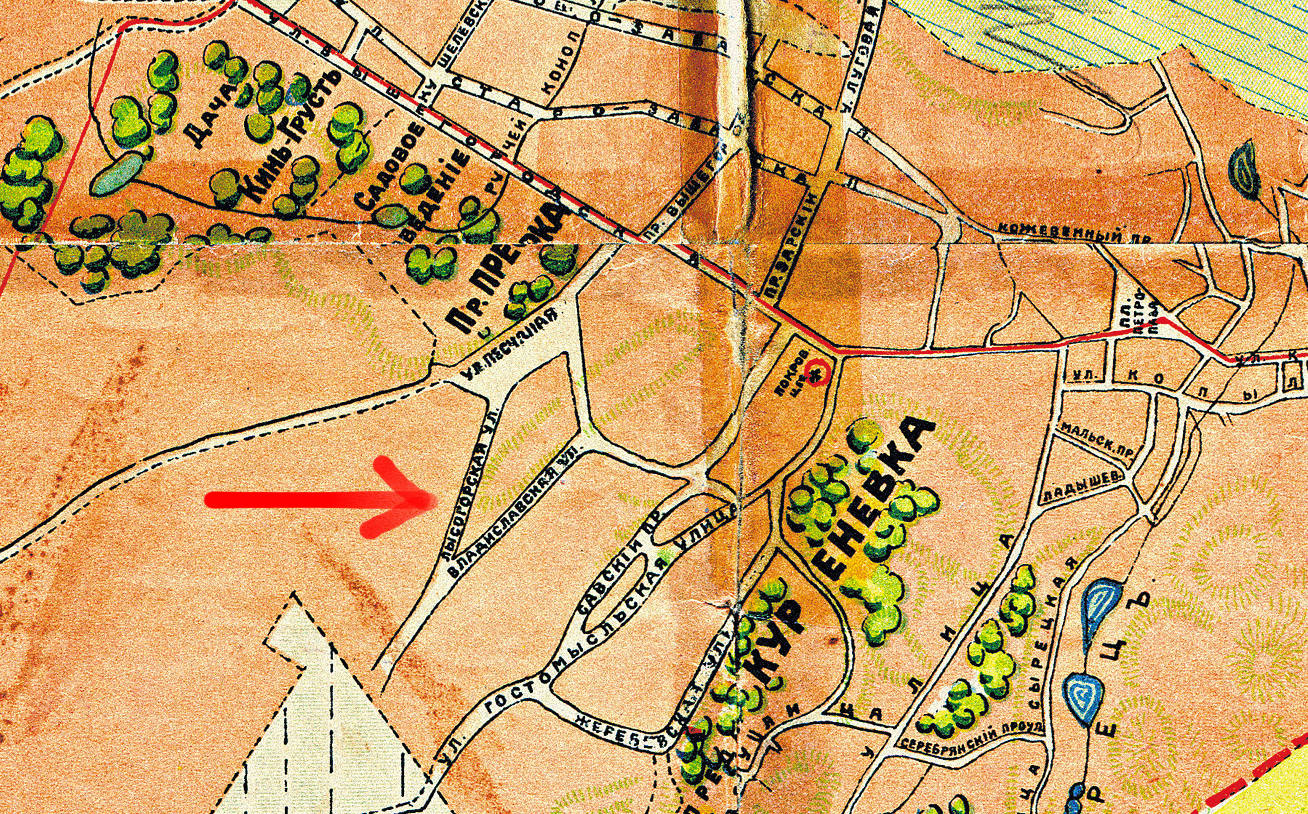
\includegraphics[width=\textwidth]{chast-lys-gory/vvedenie/1912-lys.jpg}

\textit{Кусок карты 1912 года.}
\end{center}

Вообще откуда взялись представления о шабашах? Какие-то свидетели, жившие около той или иной Лысой горы, наблюдали слёт ведьм и упырей? Или же шабаши эти, по крайней мере связанные с полетами, являлись чем-то наподобие грёзы, разделяемой множеством участников, и происходили не наяву?

Примечательно, что в быличках герой, всегда человек внешний относительно ведовского сообщества, не попадает на шабаш случайно (шел через лесок и вдруг наткнулся на шабаш), однако следует за представительницей этого сообщества, выполняя те же действия, что и она. Либо ведьма сама берет героя на шабаш. Эта закономерность прослеживается от былички к быличке и может стать ключиком к пониманию ускользающей от меня тайны.

Толковать предание о шабашах на Лысых горах можно несколькими способами.

Первый – считать всё выдумкой. 

Второй – предположить носителей технологии более развитой, чем у местного большинства. В носителей этой технологии можно записать инопланетян, пришельцев из параллельного мира, представителей ушедшей в подполье «старой» цивилизации, и так далее. И в старину седую, если бы кто летал на каком аппарате, то местом посадки выбирал бы чистую от деревьев и кустов вершину – Лысую гору. Там к нему в назначенное время или день могли бы выходить дикие туземцы и поклоняться. И шабаши на Лысых горах – не отголосок ли подобных встреч, в своё время переродившихся в отвлеченные обряды? 

Третий – ведьмы летали на Лысую гору в самом деле, физически.

Четвертый – ведьмы летали на Лысую гору в своем воображении, или каком-то разделяемом между ними сновидении\footnote{В 16-17 веках на севере Италии, во Фриули, были такие benandanti – можно перевести как «ходящие в добре», которые утверждали, что во время сна они, вместе с другими benandanti, вне своих спящих тел, летали по небу в телах мышей, кошек, бабочек и боролись с ведьмами (чтобы те не навредили урожаю), проводили между собой разные игрища, общались с некими потусторонними существами. Насколько эти сведения верны по отношению к верованиям самих benandanti – непонятно, ибо инквизиция сочла benandanti еретиками, а способы добывания сведений инквизицией широко известны.}, где место сбора соответствовало Лысой горе, существующей также и наяву. К слову, в одном из ирландских преданий, девушка, чтобы попасть на ночное гульбище эльфов, сжигала листья, вырванные из венка, подаренного ей фэйри,  вдыхая дым, впадала в транс, в котором переносилась в мир фэйри, где встречала, кроме прочего, своего умершего возлюбленного\cite{wilde01}. Обвиняемые на процессах инквизиции ведьмы говорили, что посещают шабаши как во сне, так и наяву.

Пятый – всё происходило не столь фантастически, на Лысой горе собирались остатки языческого жреческого сословия, разные «знающие люди», и проводили там свои обряды. К тому же – царская Россия, брожение религиозной мысли множества христианских ересей. Проявления многих из них вполне можно было принять за шабаши.

Однако былички ведь не про это, они описывают сложный и единственно возможный способ посещения шабаша, исключающий – образно говоря – случайную встречу в лесу.

Былички, в отличие от западных протоколов судов над ведьмами, лишены подробностей, описания происходящего на шабашах, но упорно напоминают мне завязку фильма «Гостья из будущего», когда школьник Коля Герасимов, увязавшись за странной незнакомкой, заходит в предназначенный под снос дом, видит, что женщина пользуется каким-то порталом, повторяет ее действия и переносится в будущее.

Наша быличка будто происходит из уст этого Коли Герасимова, он последовательно излагает, что с ним случилось, но в точке описания шабаша – всё, шабаш! Ничего не ясно, что же там творится. Разве что поначалу не замечают, что Коля посторонний, а дружественная к нему ведьма старается поскорее его с шабаша спровадить. Например садит на коня, и герой скачает куда-то, скачет, покуда не оказывается, что под ним не конь, а обычная палка, и предстоит еще долгий путь пешком. Многие былички про шабаши заканчиваются пробуждением героя – что роднит такие истории с опять же некоторыми рассказами про сходбища эльфов, только в последних герой чаще своими ногами приходит на какой-нибудь «холм эльфов» и там погружается в сон наяву.

В Европе, ведьмы признавались инквизиции, что летали на шабаши во сне. Однако Шпренгер и Инститорис – сочинители мерзейшей книги «Молот ведьм» – настаивали, что ведьмы могут летать и физически. А, например, документы 16 века касающиеся судов над ведьмами в Шотландии, пестрят признаниями ведьм не о шабашах, но про постоянное общение с эльфами из мира Elfame и с королевой фэйри, причем в качестве эльфов часто называются покойники, известные ведьмам при жизни.

Еще до того, как узнал про «данные инквизиции» я пришел к мысли, что шабаши происходили в сновиденческом мире. На это меня натолкнуло много закономерностей – постоянные упоминания о сне и пробуждении в быличках (герой засыпает, потом просыпается, попадает на шабаш, а потом снова просыпается), географическое положение – пожалуй, каждая Лысая гора в Киеве даже в старину была расположена поблизости от жилья, как же там могли происходить шабаши? Наяву, прилюдно не могли. Значит во сне. В каком-то ином Киеве, существующем равно как и тот, где мы живем наяву. И вот где в самом деле цветет папоротник и творятся всякие чудеса!

% И тогда возникает вопрос сновиденческого краеведения.

%, а также сами эльфы именуются gude wychtis – «хорошими ведьмами».

Ну а наяву, к концу 19 века Лысой горой стали называть и Девич-гору южнее Зверинецкого холма. На эту-то многострадальную гору и переползли в 20 и 21 веках все сопутствующие званию Лысой горы суеверия.
